\documentclass[addpoints]{exam}
\usepackage{amsmath}
\usepackage{graphbox}
\usepackage{hyperref}
\usepackage{subcaption}
\usepackage{tabularx}
\usepackage{tikz}
\usetikzlibrary{positioning}

% Header and footer.
\pagestyle{headandfoot}
\runningheadrule
\runningfootrule
\runningheader{CS 440 Computer Graphics}{Homework 2}{Spring 2018}
\runningfooter{}{Page \thepage\ of \numpages}{}
\firstpageheader{}{}{}

\qformat{{\large\bf \thequestion. \thequestiontitle}\hfill[\totalpoints\ points]}
\boxedpoints
% \printanswers

\title{Habib University\\CS 440 Computer Graphics\\Spring 2018}
\author{Homework 2, \numpoints\ points}
\date{Due: TBD}

\begin{document}
\maketitle

\begin{questions}

\titledquestion{The Prototype-Instance Paradigm}

\begin{figure}[h]
  \begin{subfigure}[b]{.33\textwidth}
    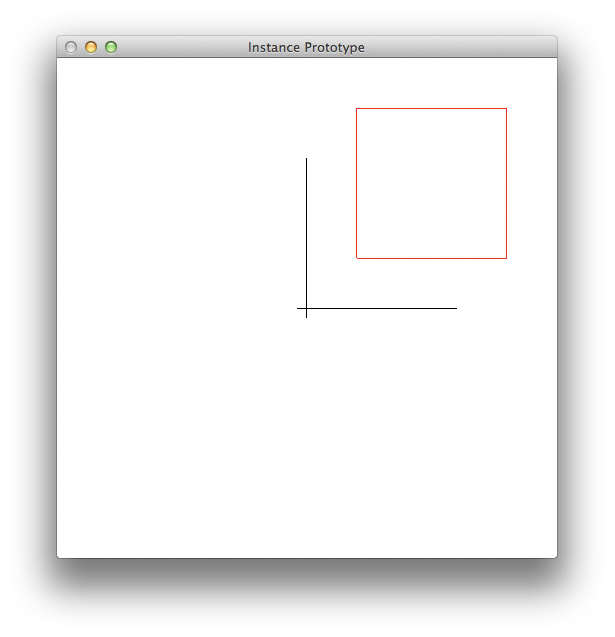
\includegraphics[width=\textwidth]{instance1}
    \caption{A prototype shape along with the x-, y- axes.}
  \end{subfigure}
  \begin{subfigure}[b]{.33\textwidth}
    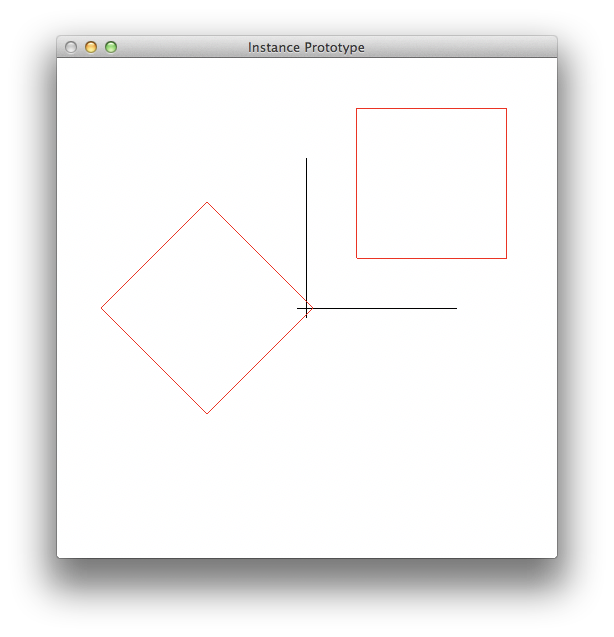
\includegraphics[width=\textwidth]{instance2}
    \caption{The prototype along with an instance.}
  \end{subfigure}
  \begin{subfigure}[b]{.33\textwidth}
    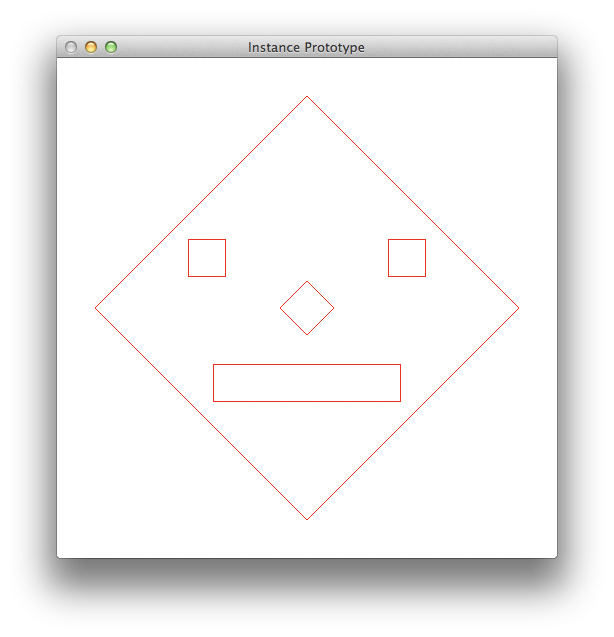
\includegraphics[width=\textwidth]{instance3}
    \caption{A face drawn using instances of the prototype.}
  \end{subfigure}
  \caption{A prototype and its instances.}
\end{figure}  

A fast and efficient transformation mechanism in OpenGL leads to the {\it prototype-instance} paradigm whereby shapes are not stored individually, instead, wherever possible, instances are generated by applying transformations to a few stored prototypes.\\
\underline{File}: {\tt instance.cpp}

  \titledquestion{Koch Snowflake}
  
  \begin{figure}
    \centering
  \begin{subfigure}[b]{.45\linewidth}
    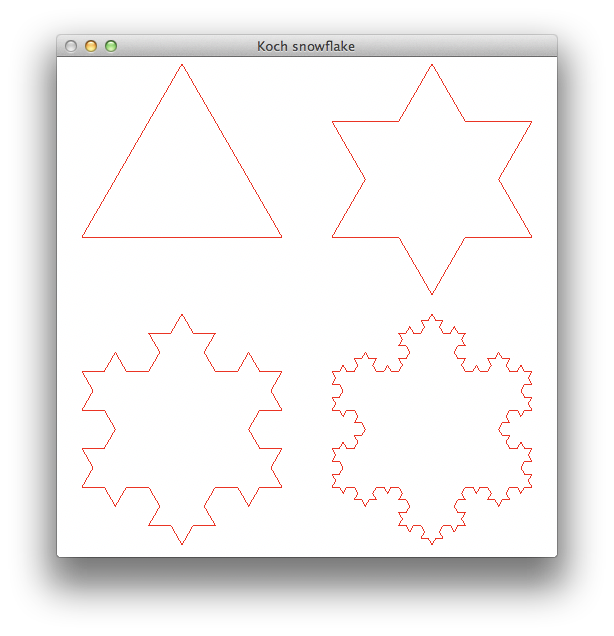
\includegraphics[width=\textwidth]{koch1}
    \caption{The first 4 iterations of the \href{https://en.wikipedia.org/wiki/Koch_snowflake}{Koch snowflake}.}
    \label{fig:koch1}
  \end{subfigure}
  \begin{subfigure}[b]{.45\linewidth}
    \raisebox{1.5\totalheight}{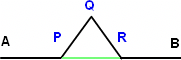
\includegraphics{koch2}}
    \caption{The recursive step.}
    \label{fig:koch2}
  \end{subfigure}
  \caption{In every iteration, the line segment $AB$ is replaced by the polyline $APQRB$ where the length of all shown line segments is equal to $\frac{|AB|}{3}$.}
\end{figure}

The \href{https://en.wikipedia.org/wiki/Koch_snowflake}{Koch snowflake}, Figure \ref{fig:koch1}, is a \href{http://mathworld.wolfram.com/Fractal.html}{fractal} generated by repeatedly applying the same transformation,
shown in Figure \ref{fig:koch2}, to all straight lines.
\begin{parts}
\part Write a function {\tt KochLine(GLfloat A[2], GLfloat B[2])} that draws the polyline $APQRB$ by repeatedly transforming and rendering the same line segment of length $\frac{|AB|}{3}$. See the code skeleton in Table \ref{tab:koch}. Calling {\tt KochSnowflake} generates the first iteration of the Koch snowflake, where $A$, $B$ and $C$ are vertices of an equilateral triangle.
\part Add a {\tt recursion\_depth} parameter to the {\tt Koch*} functions and modify the functions accordingly such that calling {\tt KochSnowflake} with {\tt recursion\_depth} equal to $n$ produces the $n$-th iteration of the Koch snowflake. The triangle $ABC$ corresponds to $n = 0$.
\part Generate Figure \ref{fig:koch1}. A sample display function is shown in Table \ref{tab:koch}.
\end{parts}
\underline{File}: {\tt koch.cpp}

\begin{table}
  \begin{tabular}{p{.5\textwidth}|p{.45\textwidth}}
    \begin{verbatim}
void kochLine(GLfloat A[2], GLfloat B[2]) {
  // segment endpoints.
  GLfloat v0[2], v1[2];
  // begin transformations.
  glPushMatrix();

  /* Transformation magic. */
  /* Assign v0, v1; only once. */    
  drawLine(v0, v1);
  /* Transformation magic. */
  drawLine(v0, v1);
  /* Transformation magic. */
  drawLine(v0, v1);
  /* Transformation magic. */
  drawLine(v0, v1);

  // end transformations.
  glPopMatrix();
}
\end{verbatim}
    \hrule
\begin{verbatim}

void drawLine(GLfloat A[2], GLfloat B[2]) {
  glBegin(GL_LINES);
  glVertex2fv(A);
  glVertex2fv(B);
  glEnd();
}
\end{verbatim}
    &
\begin{verbatim}
void kochSnowflake(GLfloat P[2],
                   GLfloat Q[2],
                   GLfloat R[2]) {
  KochLine(P, Q, depth);
  KochLine(Q, R, depth);
  KochLine(R, P, depth);
}
\end{verbatim}
      \hrule
\begin{verbatim}
void display() {
  // GL stuff.
  // equilateral triangle
  GLfloat v[3][2] = {{5,14},
                     {25, 48.64},
                     {45, 14}};
  // begin transformations.
  glPushMatrix();

  /* Transformation magic. */
  kochSnowflake(v[0], v[1], v[2]);
  /* Transformation magic. */
  kochSnowflake(v[0], v[1], v[2]);
  /* Transformation magic. */
  kochSnowflake(v[0], v[1], v[2]);
  /* Transformation magic. */
  kochSnowflake(v[0], v[1], v[2]);

  // end transformations.
  glPopMatrix();
  glFlush();
}
\end{verbatim}
  \end{tabular}
  \caption{{\tt koch*} and {\tt display} functions for the Koch snowflake.}
  \label{tab:koch}
\end{table}  


\titledquestion{Nice Doggie}

\begin{parts}
  \part Model a 3D world with three objects (you may add more but that is not the requirement of the assignment) using simple objects like sphere/cylinder/cube etc. available as OpengGL functions (or you may want to make your own routines).
\begin{enumerate}
\item A dog with at least the following parts visible: four legs, a tail, nose, eyes and ears. Each leg will have three joints, one between leg/body, one joint between the leg/paw and one with upper/lower leg.
\item A ball
\item A bone
\end{enumerate}
The initial positions of these objects can be arbitrary but for simplicity keep both the objects in front of the dog in easy reach as it would simplify your solution to the next part).
\part Your static dog from the previous part is alive now (virtually, that is). You give instructions (through keyboard/mouse) and your pet follows them. How good its behaves depends on your training (programming). The minimum set of instructions to qualify your dog as ``well-behaved'' are: walk, wag tail, kick ball, pick bone, and stop doing the action previously given.
\end{parts}
\underline{File}: {\tt doggie.cpp}

\titledquestion{The Mandelbrot Set}

\begin{table}
  \centering
  \[\begin{array}{l||c|c||c|c}
      n & z_n(3+4\iota) & |z_n(3+4\iota)| & z_n(-0.5-0.5\iota) & |z_n(-0.5-0.5\iota)|\\\hline
      0 & 0\iota & 0.0 & 0\iota & 0.0\\
      1 & 3+4\iota & 5.0 & -0.5-0.5\iota & 0.7071067811865476\\
      2 & -4+28\iota & 28.284271247461902 & -0.5+0\iota & 0.5\\
      3 & -765-220\iota & 796.0056532462568 & -0.25-0.5\iota & 0.5590169943749475\\
      4 & 53628+336604\iota & 633629.6666034507 & -0.6875-0.25\iota & 0.7315437444199766
    \end{array}
  \]
  \caption{The values and magnitudes of $z_n$ for two different complex numbers. Until $n = 4$, $z_n$ escapes for one number and not for another.}
  \label{tab:mandel}
\end{table}

\begin{figure}
  \centering
  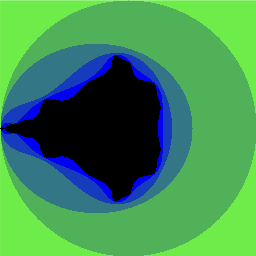
\includegraphics[width=.24\textwidth]{mandel1}
  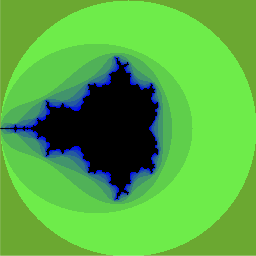
\includegraphics[width=.24\textwidth]{mandel2}
  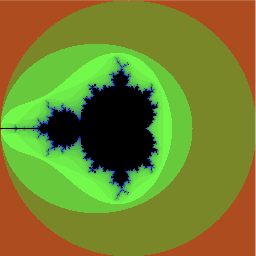
\includegraphics[width=.24\textwidth]{mandel3}
  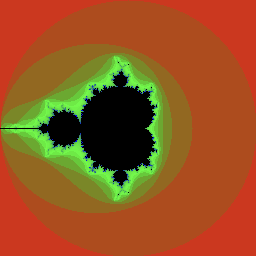
\includegraphics[width=.24\textwidth]{mandel4}
  \caption{Mandelbrot images for {\tt limit} = 5, 10, 25, and 50. The images visualize the part of the complex plane in $[-2,2)$ on the real (horizontal) axis and $[-2,2)$ on the imaginary (vertical) axis. Points in black are members of the Mandelbrot set. Other colors indicate how far ago in the past a point escaped. Red is oldest and Blue is newest, with Green in the middle.}
  \label{fig:mandel}
\end{figure}

The \href{https://en.wikipedia.org/wiki/Mandelbrot_set}{Mandelbrot set} is a popular fractal. It is defined mathematically using the series, $z_n$, which is computed using a complex number, $c$, and a positive integer, $n$, as
\[
  z_n(c) = \begin{cases}
    0 & n=0\\
    z_{n-1}^2(c)+c & \textrm{otherwise}
  \end{cases}
\]
For some values of $c$, the {\it modulus} of $z_n$, denoted as $|z_n|$, becomes larger and larger as $n$ increases, i.e. $z_n$ {\it escapes to infinity}. The Mandelbrot set, $M$, is the set of all complex numbers, $c$, such that $z_n$ does not escape to infinity. See Table \ref{tab:mandel} for an example.

When computing the elements of $M$, the following property of non-elements of $M$ proves especially helpful. The magnitude of $z_n(c)$ for every $c$ that escapes to inifinity becomes larger than 2 at some value of $n$. That is,
\[
  (\exists n_0: |z_{n_0}(c)| > 2) \implies (c \not\in M).
\]
$n_0$ is called the {\it escape time} of $c$.
The above equaltion also yields,
\[
  \forall c\in M: (-2\leq Re(c)\leq 2) \land (-2\leq Im(c)\leq 2)
\]
\begin{parts}
  \part Write a function, {\tt escapeTime}, that takes $n$ and $c$ as arguments and returns the escape time of $c$ up to $n$. That is, if the escape time is greater than $n$ then the function returns -1. Otherwise, it returns the escape time.
  \part Write a function, {\tt inMandelBrot}, that takes $n$ and $c$ as arguments and returns {\tt True} if $c$ does not escape until $n$ and {\tt False} otherwise.
  \part We will now visualize the Mandelbrot set, e.g. Figure \ref{fig:mandel}. We generate complex numbers $c_i$ such that $Re(c_i) \in [−2, 2)$ and $Im(c_i) \in [−2, 2)$, and each $c_i$ can be mapped exactly to a pixel in a 256x256 image. For a specified {\tt limit}, each $c_i$ is checked for its escape time and the corrsponding pixel is colored accordingly. The images in Figure \ref{fig:mandel} are obtained by assigning colors as follows.
  \begin{itemize}
  \item black: members of $M$, i.e. values of $c_i$ that do not escape till {\tt limit}) 
  \item blue: values of $c_i$ whose escape value is close to {\tt limit}
  \item red: values of $c_i$ whose escape value is close to {\tt 0}
  \item green: values of $c_i$ whose escape value is between 0 and {\tt limit}.
  \end{itemize}
  Write the function {\tt visualizeMandelbrot(int limit)} that generates the image as described. You may use a different color scheme than the one used in Figure \ref{fig:mandel}.  
\end{parts}
\underline{File}: {\tt mandelbrot.cpp}

\end{questions}

\end{document}



